\documentclass[11pt]{article}

\marginparwidth 0.5in 
\oddsidemargin 0.25in 
\evensidemargin 0.25in 
\marginparsep 0.25in
\topmargin 0.25in 
\textwidth=6in
\textheight=8in

\usepackage{indentfirst} % indents all paragraphs
\usepackage{graphicx}
\usepackage{subcaption}
\usepackage{pgffor}
\usepackage{hyperref}

\begin{document}
\hfill\vbox{\hbox{Jude Shin}
		\hbox{CSC 4888-S01}	
		\hbox{Lab 8.3: Structure from Motion}	
		\hbox{\today}}\par

\bigskip
\centerline{\Large\bf Colmap Experiment}\par
\bigskip

As you can see in Figure~\ref{fig:3dscreen}, With more images, there are more points that were plotted.
I decided to try and make different .obj files using 10 and 19 images.
The colmap application that I used can be found \href{https://offlinetools.io/colmap/}{here}.
I decided to use the default 200px thumbnails with exhaustive keypoint matching.
This is still not as good as I would like it to be. 
It would be nice if we could just take all the frames from a video and construct the objects from there.

It seems like a lot of the table was mapped (a lot of the brown dots in a line were mapped).
The smooth surface of the bag made it hard to extract key-points, so only light blue from the text or zipper seemed to show up.
I probably would have gotten better results if I took a picture of the scene or something.

\begin{figure}[htbp]
    \centering
    % Loop from image 1 to 9
    \foreach \i in {1,...,19}{%
        \begin{subfigure}[b]{0.14\textwidth}
            \centering
            % Assumes your images are named 1.jpg, 2.jpg, etc.
            \includegraphics[width=\textwidth]{assets/bag/img\i.png}
						% \caption{Image \i}
        \end{subfigure}%
        %
        % Automatically break row every 3 images (when \i is a multiple of 3)
        \ifnum\numexpr\i\relax=5 \\ \vspace{1em} \fi
        \ifnum\numexpr\i\relax=10 \\ \vspace{1em} \fi
        \ifnum\numexpr\i\relax=15 \\ \vspace{1em} \fi
        \ifnum\numexpr\i\relax=20 \\ \vspace{1em} \fi
        % If it's not a row break, add a horizontal fill space
        \ifnum\numexpr\i\relax=5\else
          \ifnum\numexpr\i\relax=10\else
            \ifnum\numexpr\i\relax=15\else\hfill
							\ifnum\numexpr\i\relax=20\else\hfill\fi
						\fi
          \fi
        \fi
    }%

    \caption{All images used.}
    \label{fig:imageGrid}
\end{figure}

\clearpage

\begin{figure}[h!]
	\centering
	\begin{subfigure}{0.45\textwidth}
		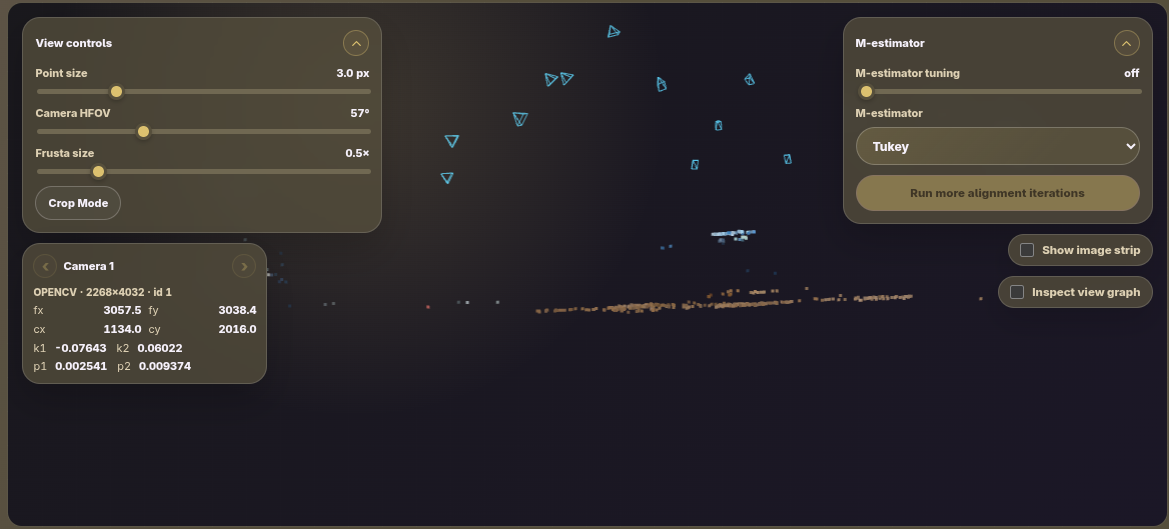
\includegraphics[width=\textwidth]{assets/colmap_19_pts.png}
		\caption{Map using 19 images.}
		\label{fig:sub-a}
	\end{subfigure}
	\hfill
	\begin{subfigure}{0.45\textwidth}
		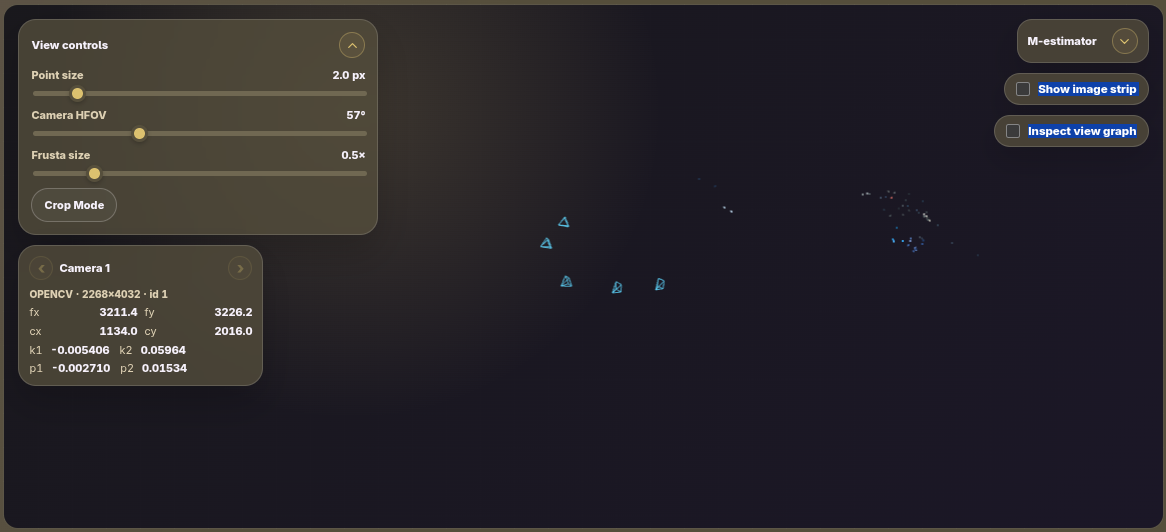
\includegraphics[width=\textwidth]{assets/colmap_10_pts.png}
		\caption{Map using 10 images.}
		\label{fig:sub-b}
	\end{subfigure}
	\caption{Significantly more detail with the mapping from more images.}
	\label{fig:3dscreen}
\end{figure}

\end{document}
